Reducing the dimensionality of $A$ with an OSE is a promising approach,
and is used in practice. 
Define
\begin{align*}
    % \norm{b - A\tilde{w}} \leq (1+\epsilon) \norm{b - Aw^*} \\
    \tilde{w} = \argmin_{w \in \rea^n} \norm{\Pi Aw - \Pi b}^2.
\end{align*}
It was shown by \cite{sarlos2006improved} that:
\begin{claim}
\label{claim_1}
    If $m=\Omega(\epsilon^{-2})$, then with probability at least $2/3$, 
    \begin{align}
    \norm{\Pi b - \Pi A\tilde{w}} \leq (1+\epsilon) \norm{b - Aw^*}
    \end{align}
\end{claim}
%
\begin{claim}
    \label{claim_2}
    If $m=\Omega(\epsilon^{-1}d\log(d))$, then with probability at least $1/3$,
    \begin{align}
    \norm{b - A\tilde{w}} \leq (1+\epsilon) \norm{b - Aw^*}
    \end{align}
\end{claim}
%
% \begin{claim}
%     If $m=\Omega(\epsilon^{-2}d\log(d))$, then with probability at least $1/3$,
%     \begin{align}
%     \norm{w^* - \tilde{w}} \leq \epsilon \cdot \frac{\norm{b - Aw^*}}{\sigma_{\min}(A)}
%     \end{align}
% \end{claim}
%
Claim~\ref{claim_1} follows directly from the Distributional JL Lemma.
\begin{proof}(of Claim~\ref{claim_1})
Simply apply the JL transform $\Pi$ to $b - Aw^*$.
\begin{align*}
    \norm{\Pi b - \Pi A\tilde{w}} = \norm{\Pi(b - A\tilde{w})} &\leq \norm{\Pi(b - Aw^*)} \\
        &\leq (1+\epsilon) \norm{b - Aw^*}
\end{align*}
\end{proof}
However, Claim~\ref{claim_1} is not a terribly interesting result. 
It simply states that the error in the embedded space, 
is close to the error in the original space.
From the standpoint of bounding the error of the approximate solution,
Claim~\ref{claim_2} is much more useful.
Since this tells us about the error of the approximate solution
when applied in the original space,
which is the problem we actually care about. 

Intuitively, if we embed the whole $(d+1)$ dimensional 
subspace spanned by the columns of $A$ and the vector $b$,
then we preserve the optimization problem.
This is confirmed formally in \cite[p31]{DBLP:journals/corr/Woodruff14},
although this author questions his proof approach in Appendix~\ref{app:question}.
According to Lemma~\ref{lem:subspace_ext},
embedding this subspace should require $m=\calO(\epsilon^{-2}d\log(d/\epsilon)$ dimensions.
The relaxation to the $\epsilon^{-1}$ dependence in Claim~\ref{claim_2} is not immediately obvious. 
The key to its proof is to use the \textit{normal equations},
i.e., the exact solution to the linear regression mentioned above,
\begin{align}
\label{eq:normal_eq}
    w^* = (A^T A)^{-1}A^T b.
\end{align}
From these equations we note that
\begin{align*}
    A^T A w^* - A^T b &= 0 \\
    A^T(A w^* - b) &= 0,
\end{align*}
i.e., $(A w^* - b)$, the residual vector,
is orthogonal to the columns of $A$.
As such, $(A \tilde{w} - b)$ can be written as the sum of two orthogonal vectors,
$(A w^* - b)$ and $(A \tilde{w} - A w^*)$.
We can then use the Pythagorean theorem to note,
\begin{align}
\label{eq:pythagorus}
\norm{A \tilde{w} - b}^2 = \norm{A w^* - b}^2 + \norm{A \tilde{w} - A w^*}^2.
\end{align}
The proof thus only needs to show that $\norm{A \tilde{w} - A w^*}^2 = \calO(\epsilon)\norm{A w^* - b}^2$.
After an appropriate constant factor rescaling of epsilon, this implies
\begin{align*}
\norm{A \tilde{w} - b} &= \sqrt{(1 + \epsilon)}\norm{A w^* - b} \\
                           &\leq (1 + \epsilon)\norm{A w^* - b},
\end{align*}
i.e., we get Claim~\ref{claim_2}.

By taking this approach,
we do not need the embedding to preserve the entire subspace of $\{ \text{colspan}(A) \cup b \}$,
but rather just need it to bound a few specific terms.
One such term requires only a fixed error embedding,
the other term involves an embedding with error that is square root in $\epsilon$,
thus reducing the bound to a $\epsilon^{-1}$ requirement.
For the complete proof, 
we direct the reader to \cite{sarlos2006improved} or \cite[p33]{DBLP:journals/corr/Woodruff14}.

\begin{figure}
    \centering
    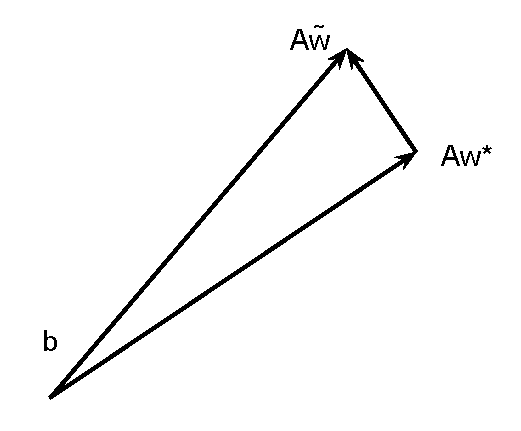
\includegraphics[width=3in]{figures/Pythogorus.pdf}
    \caption{Visualization of the vectors in Equation~\ref{eq:pythagorus}.}
    \label{fig:pythogorus}
\end{figure}